\documentclass[english,compress]{beamer} %,handout
\usepackage{amsmath}
\usepackage{graphicx}
\usepackage{biblatex}
\bibliography{references}
\usepackage{listings}
\makeatletter
%\usetheme{Boadilla}
\usetheme{Warsaw}
\setbeamertemplate{footline}
{
  \leavevmode%
  \hbox{%
  \begin{beamercolorbox}[wd=.333333\paperwidth,ht=2.25ex,dp=1ex,center]{author in head/foot}%
\usebeamerfont{author in head/foot}\insertshortauthor~~(\insertshortinstitute)
  \end{beamercolorbox}%
  \begin{beamercolorbox}[wd=.333333\paperwidth,ht=2.25ex,dp=1ex,center]{title in head/foot}%
\usebeamerfont{title in head/foot}\insertshorttitle
  \end{beamercolorbox}%
  \begin{beamercolorbox}[wd=.333333\paperwidth,ht=2.25ex,dp=1ex,right]{date in head/foot}%
\usebeamerfont{date in head/foot}\insertshortdate{}\hspace*{2em}
\insertframenumber{} / \inserttotalframenumber\hspace*{2ex} 
  \end{beamercolorbox}}%
  \vskip0pt%
}
\setbeamercovered{transparent}
\defbeamertemplate{description item}{align left}{\insertdescriptionitem\hfill}
\usecolortheme[RGB={23,51,104}]{structure}

\usepackage{babel}
%\useoutertheme{infolines}
\setbeamertemplate{headline}
{%
  \leavevmode%
  \begin{beamercolorbox}[wd=.5\paperwidth,ht=2.5ex,dp=2ex]{section in head/foot}%
    \hbox to .5\paperwidth{\hfil\insertsectionhead\hfil}
  \end{beamercolorbox}%
  \begin{beamercolorbox}[wd=.5\paperwidth,ht=2.5ex,dp=2ex]{subsection in head/foot}%
    \hbox to .5\paperwidth{\hfil\insertsubsectionhead\hfil}
  \end{beamercolorbox}%
  \vskip0pt%
}

\begin{document}

\title[Master Thesis]{BlkKin: A Low-overhead tracing infrastructure \\
for software-defined storage systems}

\author{Marios-Evangelos Kogias}
\institute[CSLab NTUA]
{
  National Technical University of Athens \\
  School of Electrical and Computer Engineering
}

\begin{frame}{Zipkin UI}
\begin{center}
 \makebox[\textwidth][c]{
        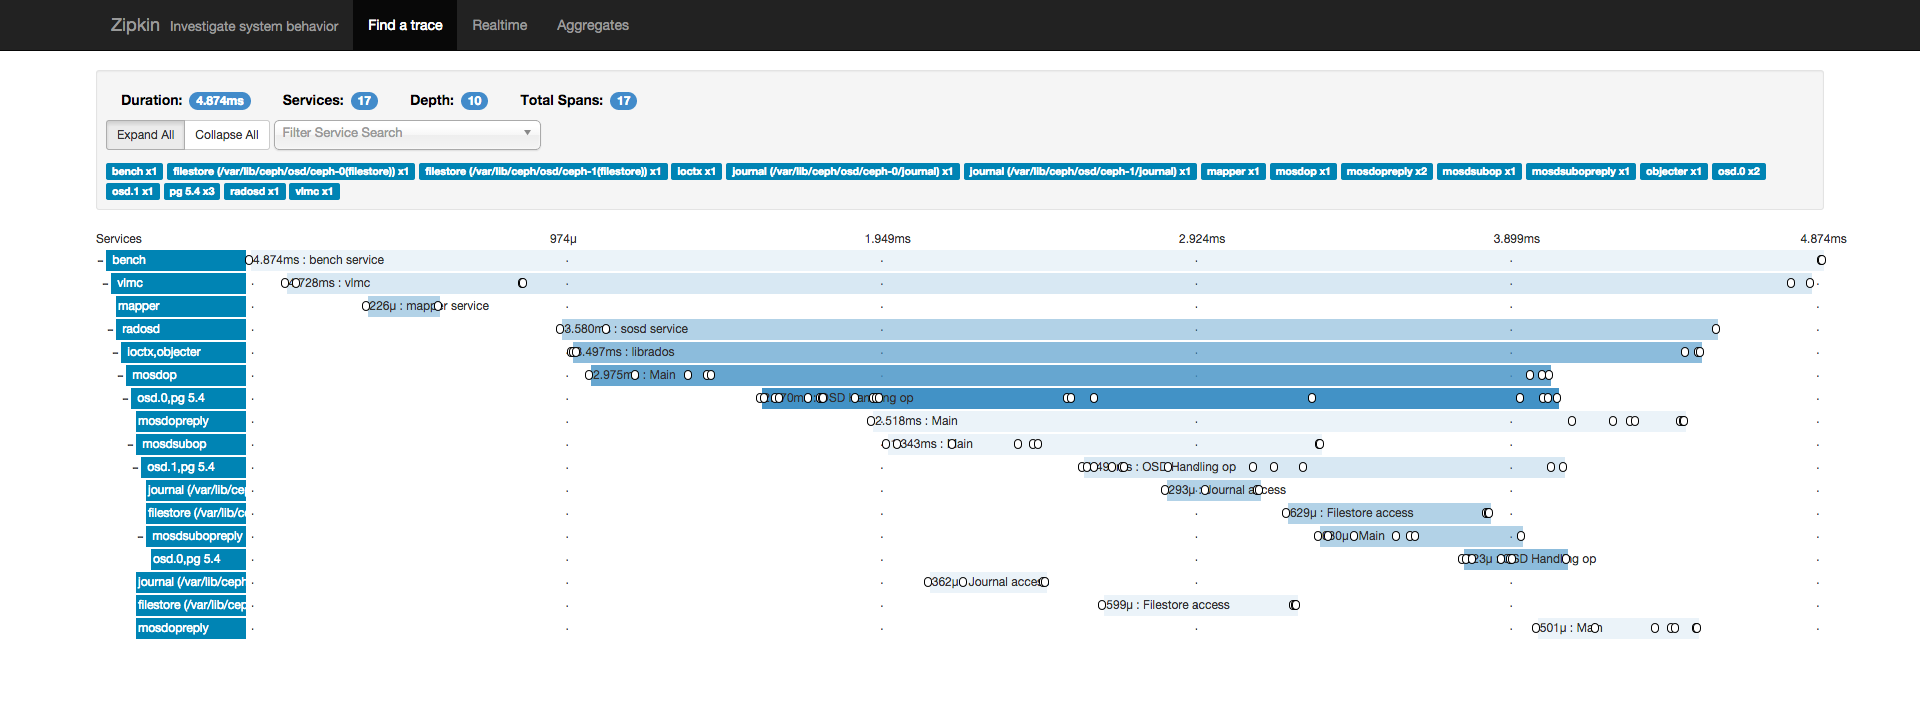
\includegraphics[width=\paperwidth]{images/zipkin-overview.png}
}
\end{center}
\end{frame}

\begin{frame}{Zipkin UI - Annotations}
\begin{center}
 \makebox[\textwidth][c]{
        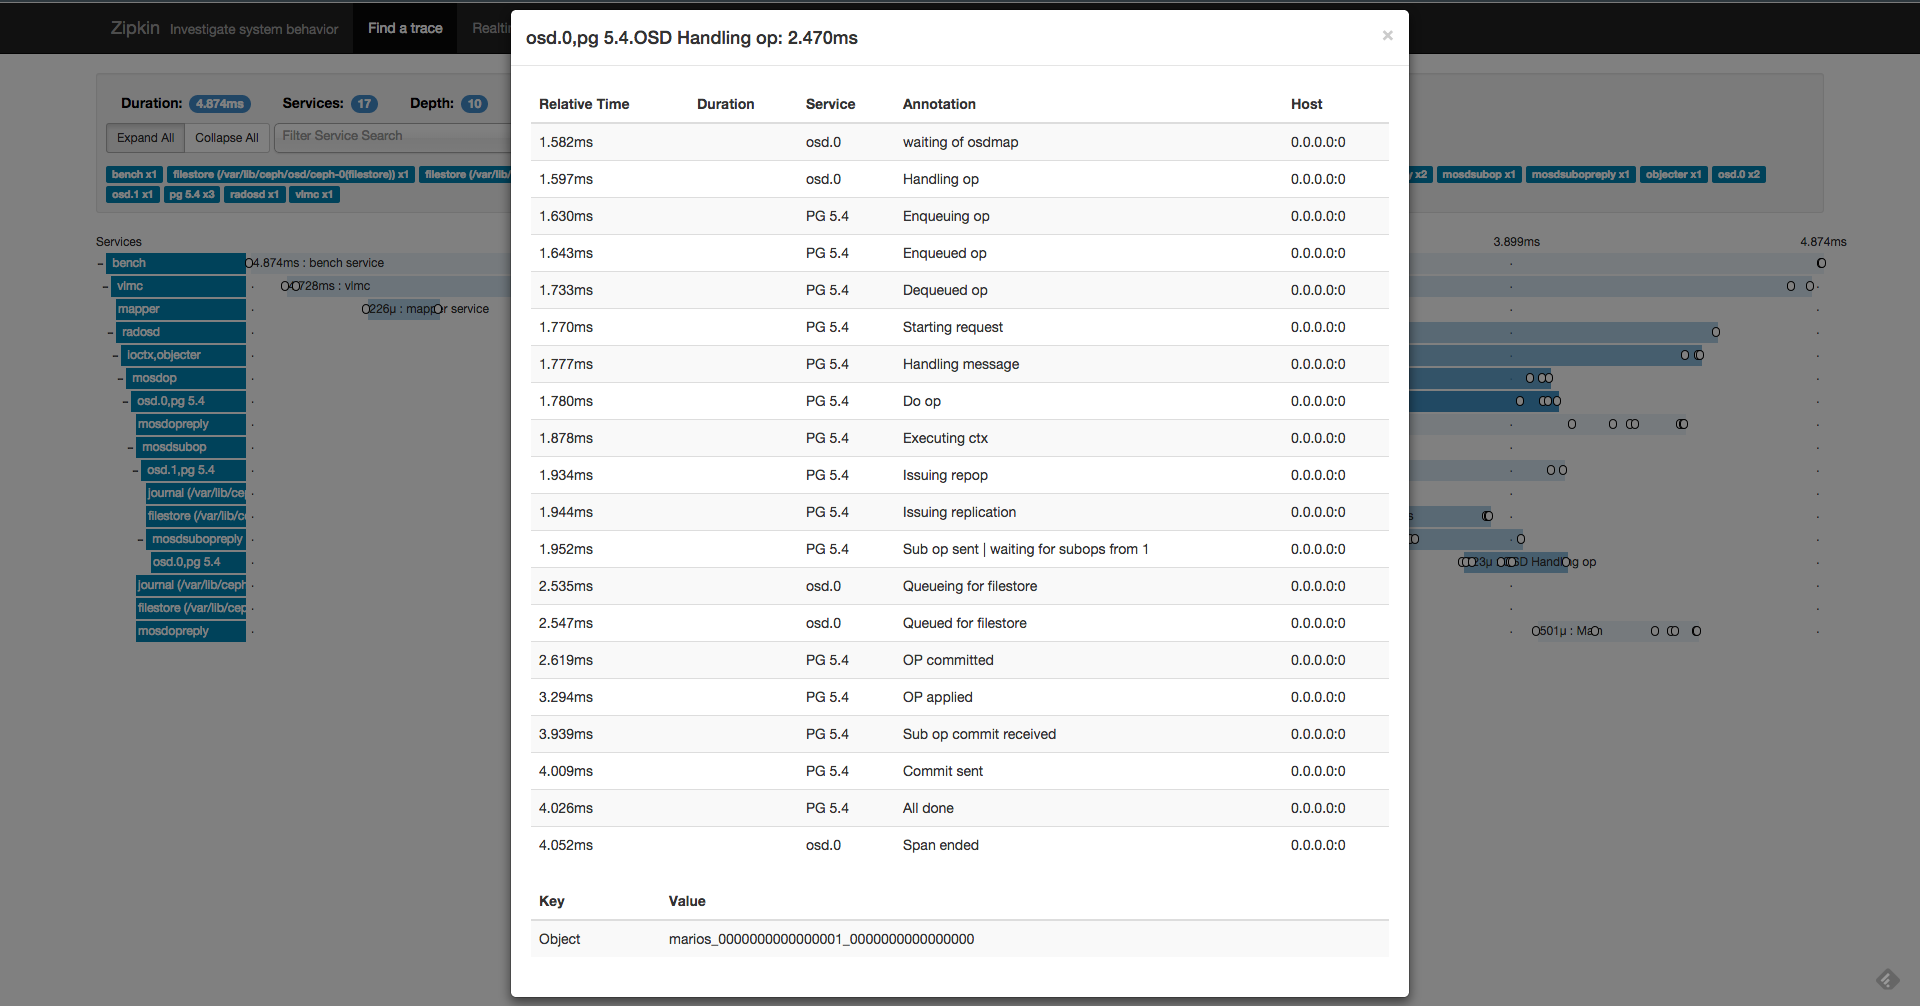
\includegraphics[width=\paperwidth]{images/zipkin-annotations.png}
}
\end{center}
\end{frame}

\begin{frame}{Zipkin UI - Dependencies}
\begin{center}
 \makebox[\textwidth][c]{
        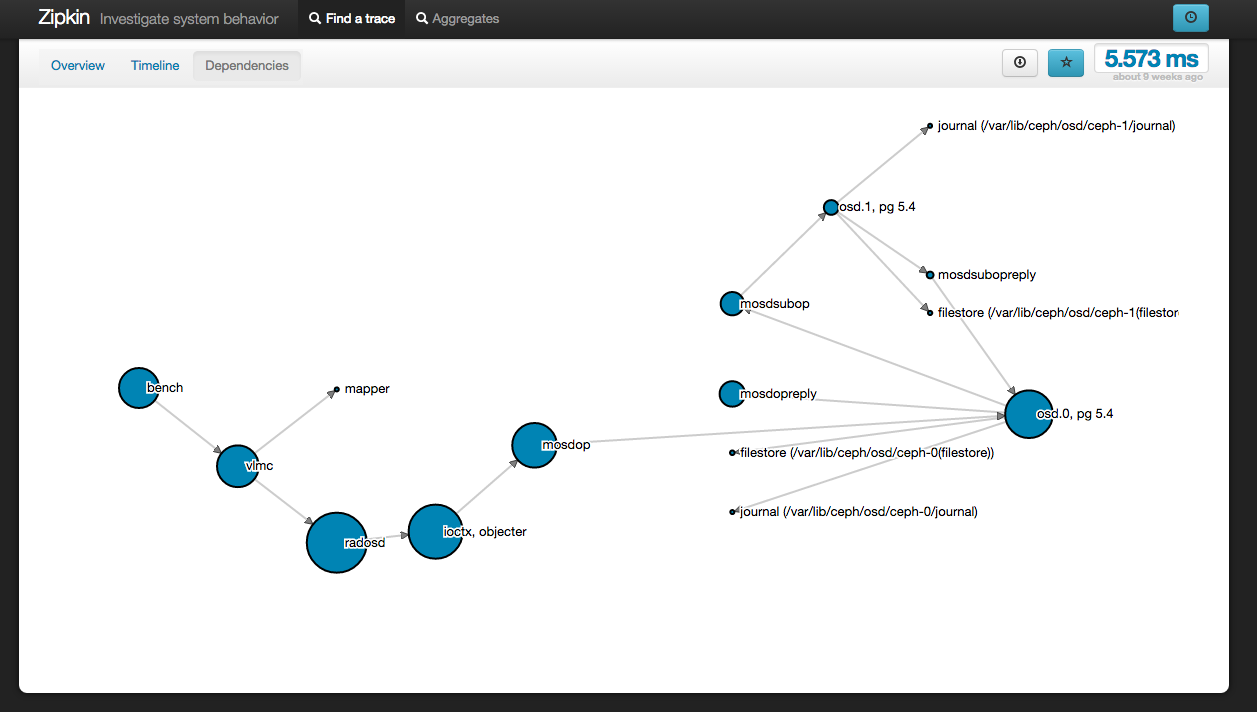
\includegraphics[width=\paperwidth]{images/zipkin-depend.png}
}
\end{center}
\end{frame}
\begin{frame}{Network fault}
\begin{center}
 \makebox[\textwidth][c]{
        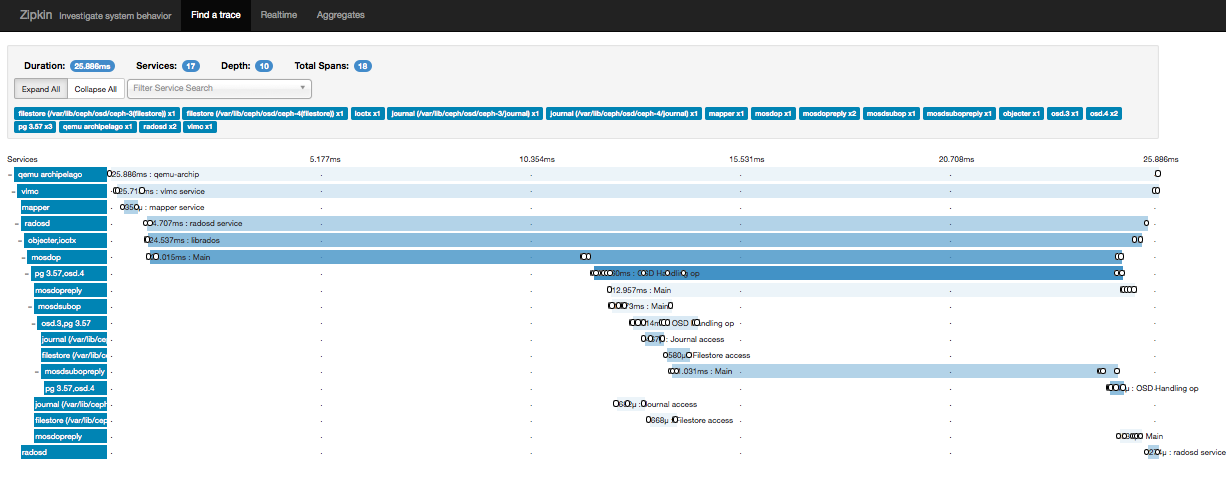
\includegraphics[width=\paperwidth,
height=0.5\paperheight]{images/network-error.png}
}
 \makebox[\textwidth][c]{
        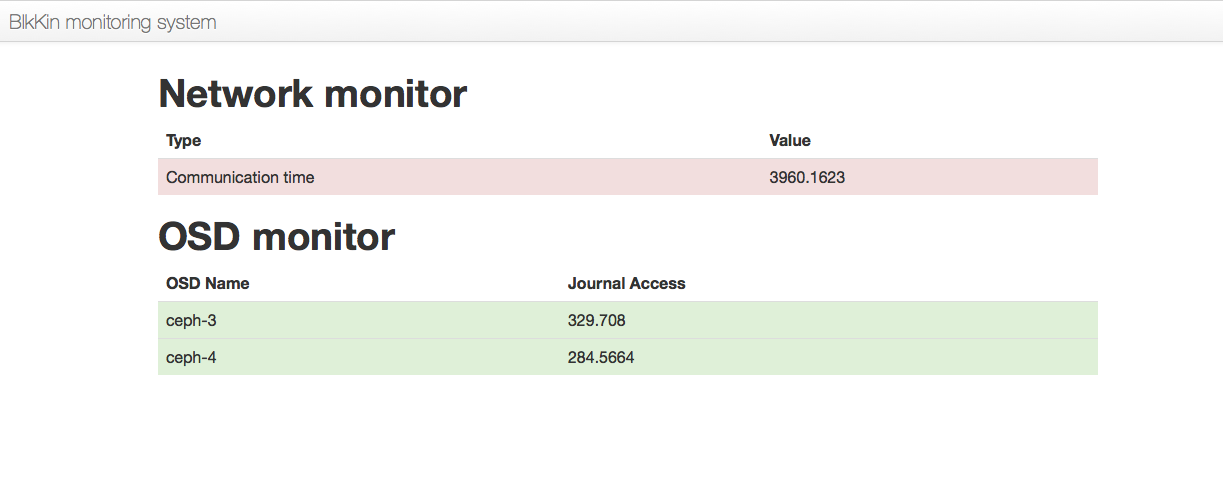
\includegraphics[width=\paperwidth,
height=0.33\paperheight]{images/network-error-blkin.png}
}
\end{center}
\end{frame}


\begin{frame}{Disk fault}
\begin{center}
 \makebox[\textwidth][c]{
        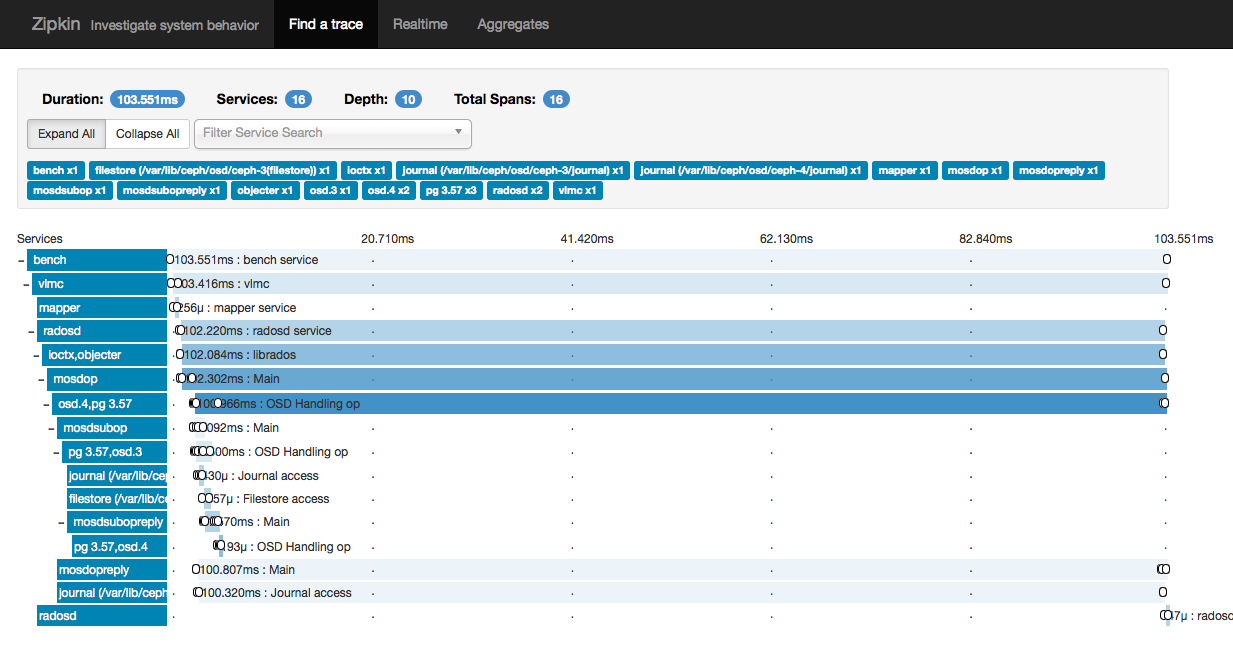
\includegraphics[width=\paperwidth,
height=0.5\paperheight]{images/disk-fault.png}
}
 \makebox[\textwidth][c]{
        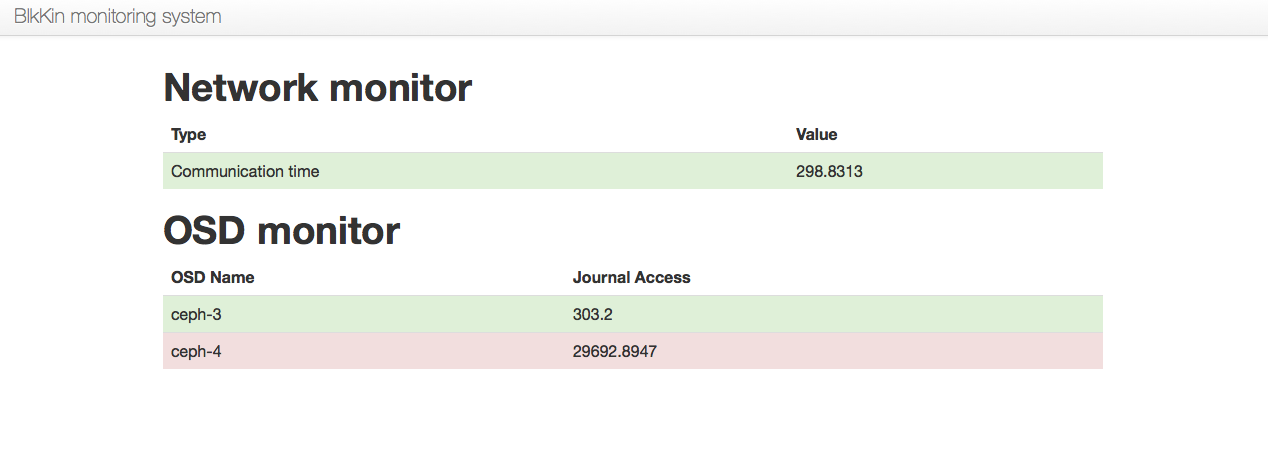
\includegraphics[width=\paperwidth,
height=0.33\paperheight]{images/disk-fault-blkin.png}
}
\end{center}
\end{frame}
\end{document}
